
The system used in the experiment is composed by a non-anthropomorphic platform and software architecture that enrich robot's movements with emotion. The robotic platform was envisioned to be as simpler as possible to let the study of the desired characteristics. 

%%%%%%%%%%%%%%%%%%%%%%%
\subsection{Hardware and Mechanical}

A holonomic platform was built to be used in the experiment. This type of platforms are characterized by the possibility to move in any direction without the necessity to have a specific orientation, i.e., they are free to move taking any desired orientation. Therefore, it was possible to imitate movements that are done by humans. For example, people move straight even if they turn their whole body a bit. The platform has a diameter of 25 cm and height of 25 cm. Figure~\ref{fig:ThirdDesign} shows the platform's blue prints and the real platform. Robot's frame of reference, in which all the velocities are going to be calculated, are depicted by the two black arrows. So, as it could be observed, to make the robot move forward it must be send a velocity in $y$ axis.

\begin{figure}
	\centering
	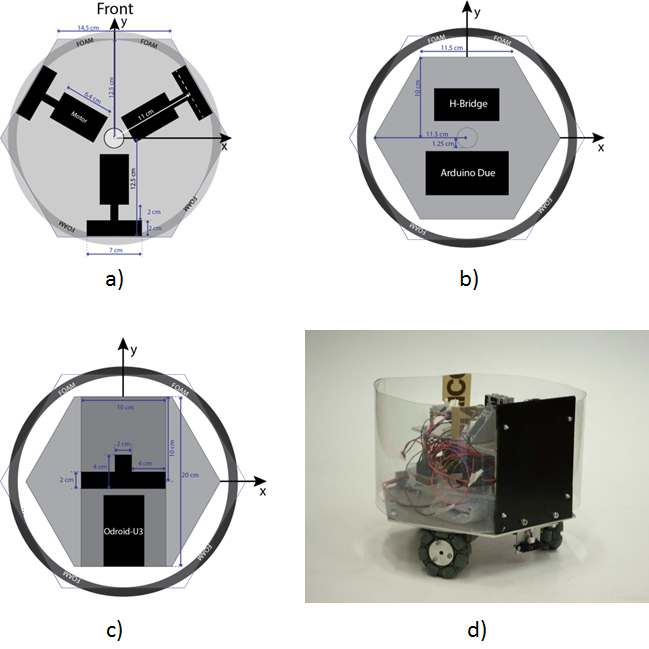
\includegraphics[width=0.48\textwidth]{Images/DesignThird.png} 
	\caption{Design of the platform. a) Base platform, this layer is used to carry the batteries. The two black arrows represent robot's frame of reference. b) First layer, which includes the Arduino and the H-Bridges to control the motors. c) Second layer with the Odroid-U3 and the mechanical structure to support the upper part. d) Lateral view of the version.}
	\label{fig:ThirdDesign}
\end{figure}

%%%%%%%%%%%%%%%%%%%%%%%platform_base
\subsection{Software}
To ensure robot's velocity it was implemented a PID controller for each motor. PID's set point is established by a controller that could receive two different types of commands. The first commands is robot's velocities ($<V_x,V_y,\omega>$), which are given in robot's frame of reference. The second command is a point ($<x, Y, \theta>$), which is given in the general frame of reference. This frame of reference is set every time the system is reset or boot. For example, if the robot finishes a trajectory and then it is reset, the new frame is going to be in the robot's current position.  

Additional to this low level control, it was created a graphical interface~\ref{fig:experimental_interface} to reduce the possibility on introducing wrong values for a desired sequence. This interface loads the sequences from a .txt file and displays sequences' numbers on it. Every time that a new sequence should be presented to a participant, the sequence's number is selected in the interface, which will display sequence's values. Once the robot has been positioned to the correct position, the execution could be started by clicking on send button. Here two commands are send, one resetting the controller and the second the desire position. In case that the sequence's execution should be aborted, it should be clicked the button stop.

\begin{figure}
	\centering
	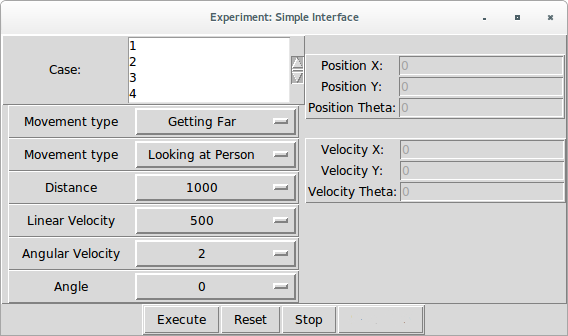
\includegraphics[width=0.45\textwidth]{./Images/ExperimentInterface.png} 
	\caption{Interface used in the experiment. Once a sequence is selected, the interface shows sequence's values. Also, the interface give information about the current position of the robot and its velocity.}
	\label{fig:experimental_interface}
\end{figure}